% Lydia Lee, lydia.lee@berkeley.edu
\qns{\textbf{(EXAM-STYLE PRACTICE)} Automatic Gain Control}

\sol{This is a design problem meant to be there \textbf{only if} students ask for exam-style practice, and as such it goes a bit beyond the standard mechanical practice/solidifying basics style CSM tends to offer. For useful amplifier topologies, see \lstinline{q_mech_nfb.tex}}

\begin{enumerate}
\qitem\label{amp}{
	Design a circuit where $V_\text{out} = -10V_\text{in}$. You are allowed to use
	\begin{itemize}
		\item op amps: $\leq$1. You do not need to specify rail voltages for this subpart.
		\item resistors: as many as you want, so long as they have positive values
		\item capacitors: as many as you want
	\end{itemize}}

\empt{
	\vspace{1cm}
	\begin{circuitikz}
		\draw
		(0,0) to[short] ++(-1,0)
			to[sV,v_=$V_\text{in}$] ++(0,-2)
			node[ground] () {};
	\end{circuitikz}
	\vspace{1cm}}

\ans{
	This is one possible solution:
	\begin{center}
		\begin{circuitikz}[scale=0.8, transform shape]
	\draw
	(0,0) node[op amp] (AMP) {}
	(AMP.-) to[short] ++(0,1) coordinate (topLeft)
		to[R,l=$10R$] (topLeft -| AMP.out)
		to[short] (AMP.out)
		to[short,-o] ++(1,0)
		to[open,o-o,v^=$V_\text{out}$] ++(0,-2)
		node[ground] () {}
	(AMP.-) to[R,l_=$R$] ++(-2,0)
		to[sV,v_=$V_\text{in}$] ++(0,-2)
		node[ground] () {}
	(AMP.+) to[short] ++(0,-1)
		node[ground] () {};
\end{circuitikz}
	\end{center}}

\qitem\label{no_rail}{
	Your design was provided voltage rails at $5\si{\volt}$ and $-5\si{\volt}$, and that your input signal looks like so:
	\begin{center}
		\begin{tikzpicture}[scale=0.75, transform shape]
\begin{axis}[
    axis lines = middle,
    ylabel = {$V_\text{in}(t)$},
    xtick={0,1.57,3.14,4.71,6.28, 7.85, 9.42, 11.00, 12.57},
    xticklabels={$0$, $\frac{\pi}{2}$,$\pi\,$,$\,\,\,\frac{3}{2}\pi$,$\,\,\,2\pi$, $\frac{5}{2}\pi$, $3\pi$, $\frac{7}{2}\pi$, $4\pi$},
    ytick={0,-0.5,0.5,-1,1},
    ymin=-1.5,
    ymax=1.5,
    xmin = 0,
    xmax=4*pi
]
\addplot [
	color=black,
	domain=0:4*pi,
	samples=200
	]
	{ 0.5*sin(deg(x))
	};
\end{axis}
\end{tikzpicture}
	\end{center}
	Will your signal be faithfully amplified when $V_\text{out} = -10V_\text{in}$, or will it rail/clip?}

\empt{\vspace{1.5cm}}

\ans{
	The signal will be faithfully amplified.

	Our output is going to be limited to $\pm 5\si{\volt}$, meaning that with an amplifier gain $\frac{V_\text{out}}{V_\text{in}} = 10$, we can have an input no larger than $0.5\si{\volt}$ in the positive or negative direction.}

\qitem\label{yes_rail}{
	Again, your design has voltage rails at $\pm 5\si{\volt}$. Your input signal now looks like so:
	\begin{center}
		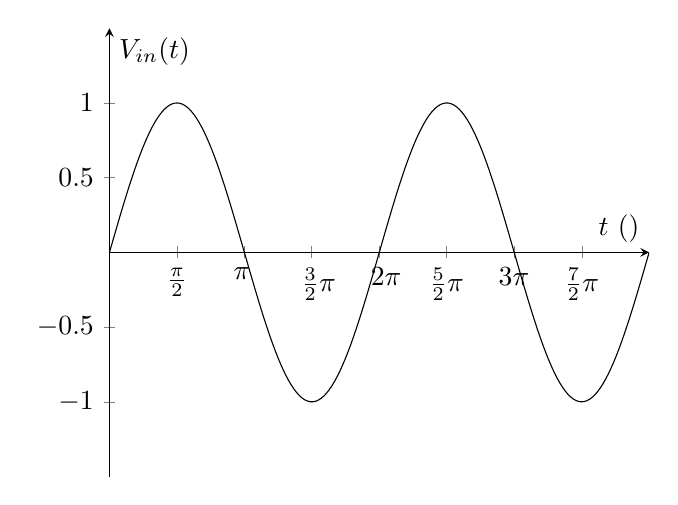
\begin{tikzpicture}
\begin{axis}[
    axis lines = middle,
    xlabel = {$t$ $(\si{\milli\second})$},
    ylabel = {$V_\text{in}(t)$},
    xtick={0,1.57,3.14,4.71,6.28, 7.85, 9.42, 11.00, 12.57},
    xticklabels={$0$, $\frac{\pi}{2}$,$\pi\,$,$\,\,\,\frac{3}{2}\pi$,$\,\,\,2\pi$, $\frac{5}{2}\pi$, $3\pi$, $\frac{7}{2}\pi$, $4\pi$},
    ytick={0,-0.5,0.5,-1,1},
    ymin=-1.5,
    ymax=1.5,
    xmin = 0,
    xmax=4*pi
]
\addplot [
	color=black,
	domain=0:4*pi,
	samples=200
	]
	{ sin(deg(x))  
	};
\end{axis}
\end{tikzpicture}
	\end{center}
	With this input signal and $V_\text{out} = -10V_\text{in}$, will your amplifier  distort the output due to railing/clipping?}

\empt{\vspace{1.5cm}}

\ans{
	The output will experience railing. From the explanation for part \ref{no_rail}, we know our input can swing no further than $0.5\si{\volt}$, and in this case the swing is $1\si{\volt}$.}

\qitem\label{resistorDAC}{
	Design a circuit which can have a resistance $R$ when an input signal $\phi$ is high and a resistance $nR$ ($n > 1$) when $\phi$ is low. You have access to:
	\begin{itemize}
		\item ideal switches: as many as you want
		\item resistors with positive values: $\leq 2$
		\item the signal $\phi$ and its complement, $\overline{\phi}$
	\end{itemize}}

\empt{\vspace{4cm}}

\ans{
	One possible solution is to place the resistor in series and short it out when $\phi$ is high:
	\begin{center}
		\begin{circuitikz}[scale=0.8, transform shape]
	\draw
	(0,0) to[short,o-] ++(1,0) coordinate (leftSide) 
		to[R=$(n-1)R$] ++(2,0) coordinate(rightSide)
		to[R=$R$] ++(2,0)
		to[short,-o] ++(1,0)
	(leftSide) to[short] ++(0,1.5) coordinate (topLeft)
		to[spst,l=$\phi$] (topLeft -| rightSide)
		to[short] (rightSide);
\end{circuitikz}
	\end{center}

	Another possible solution is to place the resistor in parallel and place a switch in series with it to close whenever $\phi$ is high. Remember that in parallel, the resistance decreases!
	\begin{center}
		\begin{circuitikz}[scale=0.8, transform shape]
	\draw
	(0,0) to[short,o-] ++(1,0) coordinate (leftSide)
		to[R=$nR$] ++(4,0) coordinate (rightSide)
		to[short,-o] ++(1,0)
	(leftSide) to[short] ++(0,1.5)
		to[spst,l=$\phi$] ++(2,0)
		to[R=$R\left(\frac{n}{n-1}\right)$] ++(2,0)
		to[short] (rightSide);
\end{circuitikz}
	\end{center}}

\qitem\label{vga}{
	Using your answer from parts \ref{amp} and \ref{resistorDAC}, design a circuit where
	$$V_\text{out} = \begin{cases}
						-5V_\text{in} & \phi = \text{high}\\
						-10V_\text{in} & \phi = \text{low}
					\end{cases}$$}
\empt{
	\vspace{1cm}
	\begin{circuitikz}
		\draw
		(0,0) to[short] ++(-1,0)
			to[sV,v_=$V_\text{in}$] ++(0,-2)
			node[ground] () {};
	\end{circuitikz}
	\vspace{1cm}}

\ans{
	Using the symbol for a variable resistor,
	\begin{center}
		\begin{circuitikz}[scale=0.8, transform shape]
	\draw
	(0,0) node[op amp] (AMP) {}
	(AMP.-) to[short] ++(0,1) coordinate (topLeft)
		to[vR,l=$R_\text{var}$] (topLeft -| AMP.out)
		to[short] (AMP.out)
		to[short,-o] ++(1,0)
		to[open,o-o,v^=$V_\text{out}$] ++(0,-2)
		node[ground] () {}
	(AMP.-) to[R,l_=$R$] ++(-2,0)
		to[sV,v_=$V_\text{in}$] ++(0,-2)
		node[ground] () {}
	(AMP.+) to[short] ++(0,-1)
		node[ground] () {};
\end{circuitikz}
	\end{center}
	we can replace $R_\text{var}$ with our answer to part \ref{resistorDAC}.
}

\qitem\label{phi_oneSide}{
	How do we generate $\phi$? We want it to be high whenever $|V_\text{in}|$ is larger than some threshold, and low otherwise. Before jumping to absolute value, let's look at a slightly simpler problem: design a circuit whose output is
	$$\phi_\text{high-side} = \begin{cases}
								V_{DD} & V_\text{in} < -0.49\si{\volt}\\
								V_{SS} & V_\text{in} > -0.49\si{\volt}
							\end{cases}$$
	You may use:
	\begin{itemize}
		\item op amps: as many as you want
		\item ideal voltage source: $\leq 1$ in addition to the $\pm 5\si{\volt}$ voltage rails
		\item your answer to part \ref{amp}, black-boxed to take in $V_\text{in}$. You may assume it works as described in part \ref{amp}
	\end{itemize}}

\empt{
	\vspace{1cm}
	\begin{circuitikz}
		\draw
		(0,0) to[short] ++(-2,0)
			to[sV,v_=$V_\text{in}$] ++(0,-2)
			node[ground] () {};
	\end{circuitikz}
	\vspace{1cm}}


\ans{
	One possible solution:
	\begin{center}
		\begin{circuitikz}[scale=0.8, transform shape]
	\draw
	(0,0) node[op amp] (AMP) {}
	(4,-0.5) node[op amp,yscale=-1] (COMP) {}

	(AMP.-) to[short] ++(0,1) coordinate (topLeft)
		to[R,l=$10R$] (topLeft -| AMP.out)
		to[short] (AMP.out)
		to[short] (COMP.+)
	(AMP.-) to[R,l_=$R$] ++(-2,0)
		to[sV,v_=$V_\text{in}$] ++(0,-2)
		node[ground] () {}
	(AMP.+) to[short] ++(0,-1)
		node[ground] () {}
	(COMP.-) to[V=$4.9\si{\volt}$] ++(0,-2)
		node[ground] () {}
	(COMP.out) to[short,-o] ++(1,0)
		node[anchor=west] () {$\phi_\text{high-side}$};
\end{circuitikz}
	\end{center}

	Mind your polarity! Remember that part \ref{amp} has a negative relationship between its output and $V_\text{in}$.
}

\qitem\label{agc}{
	Now let's put it all together. Design a circuit which lowers the gain setting when the input swing exceeds $0.49\si{\volt}$ (we usually like to leave some wriggle room just in case). You may assume all feedback loops are infinitely fast.
	$$V_\text{out} = \begin{cases}
						-5V_\text{in} & |V_\text{in}| > 0.49\si{\volt}\\
						-10V_\text{in} & |V_\text{in}| < 0.49\si{\volt}
					\end{cases}$$
	You may use
	\begin{itemize}
		\item op amps: as many as you want
		\item switches: as many as you want
		\item resistors with positive values: as many as you want
		\item ideal voltage source: $\leq 2$, in addition to the provided rails $\pm 5\si{\volt}$
		\item your answer to part \ref{vga}, black-boxed to take in $V_\text{in}$ and $\phi$. You may assume it works as described in part \ref{vga}.
		\item a device which returns the maximum of its two inputs: $\leq 1$
		\begin{center}
			\begin{circuitikz}
				\draw (0,0) node[or port] (OR) {}
				(OR.in 1) node[anchor=east] () {$V_\text{in1}$}
				(OR.in 2) node[anchor=east] () {$V_\text{in2}$}
				(OR.out) node[anchor=west] () {$V_\text{max}$};
			\end{circuitikz}
		\end{center}
	\end{itemize}
	\textit{Hint: It may be helpful to consider the single-sided case when $V_\text{in} > 0.49\si{\volt}$ first, then only start worrying about the negative case $V_\text{in} < -0.49\si{\volt}$ afterward.}}
	

\empt{
	\vspace{3cm}
	\begin{circuitikz}
		\draw
		(0,0) to[short] ++(-1,0)
			to[sV,v_=$V_\text{in}$] ++(0,-2)
			node[ground] () {};
	\end{circuitikz}}

\sol{
	This may be a large jump for your students. If they're stumped, try prompting them in this order:
	\begin{enumerate}
		\item What component generates a high or low voltage depending on which input is larger/smaller? (Almost like we're going to \textit{compare} the inputs)
		\item What would we do if we only wanted to change the gain setting when $V_\text{in} > 0.49\si{\volt}$ and not worry about the negative case?
		\item How about the negative-only case, i.e. when $V_\text{in} < -0.49\si{\volt}$?
		\item How can we combine these?
	\end{enumerate}}

\ans{
	One possible solution:
	\begin{center}
		\begin{circuitikz}[scale=0.8, transform shape]
	\draw
	(0,0) node[op amp] (AMP) {}
	(5,-2.5) node[op amp,yscale=-1] (COMP_HI) {}
	(5,2.5) node[op amp] (COMP_LO) {}
	(9,0) node[or port] (OR) {}
	(AMP.-) to[short] ++(0,1) coordinate (topLeft)
		to[vR,l=$R_\text{var}$] (topLeft -| AMP.out)
		to[short] (AMP.out)
		to[short] ++(1,0) coordinate (connector)
	(connector) to[short] (connector |- COMP_HI.+)
		to[short] (COMP_HI.+)
	(connector) to[short] (connector |- COMP_LO.-)
		to[short] (COMP_LO.-)
	(AMP.-) to[R,l_=$R$] ++(-2,0)
		to[sV,v_=$V_\text{in}$] ++(0,-2)
		node[ground] () {}
	(AMP.+) to[short] ++(0,-1)
		node[ground] () {}
	(COMP_HI.-) to[V=$4.9\si{\volt}$] ++(0,-2)
		node[ground] () {}
	(COMP_LO.+) to[V=$-4.9\si{\volt}$] ++(0,-2)
		node[ground] () {}
	(COMP_HI.out) to[short] (COMP_HI.out |- OR.in 2)
		to[short] (OR.in 2)
	(COMP_LO.out) to[short] (COMP_LO.out |- OR.in 1)
		to[short] (OR.in 1)
	(OR.out) node[anchor=west] () {$\phi$}
	(AMP.out) to[short,-o] ++(1,0)
		node[anchor=west] () {$V_\text{out}$};
\end{circuitikz}
	\end{center}
	Note that this solution is aggressive and minimal.}
\end{enumerate}

\empt{\newpage}